\section{Les réseaux d’entreprise}
\subsection{Mise en œuvre du site principal de l’entreprise}

\subsubsection{Mise en place du réseau et du service d'adressage dynamique}

L'architecture du site principal est déployée via des conteneurs (sous Containerlab) simulant les équipements réseau. Le routage inter-VLAN est assuré par un nœud Linux faisant office de cœur de réseau (\texttt{ENT-SITE-PRIM-COR-01}), qui segmente logiquement le trafic selon le plan d'adressage suivant :

\begin{table}[ht!]
    \centering
    \renewcommand{\arraystretch}{1.3}
    \begin{tabular}{|c|l|c|p{7.5cm}|}
        \hline
        \textbf{VLAN} & \textbf{Nom} & \textbf{Sous-réseau} & \textbf{Rôle / Équipements} \\
        \hline
        \textbf{10} & Datacenter & 192.168.10.0/24 & Hébergement des serveurs (Web, DNS, VoIP) en adressage statique. \\
        \hline
        \textbf{20} & Clients & 192.168.20.0/24 & Accueil des postes utilisateurs (ex : \texttt{PC-01}). \\
        \hline
        \textbf{30} & Téléphonie & 192.168.30.0/24 & Connexion des terminaux VoIP (ex : \texttt{PHONE-01}, \texttt{PHONE-02}). \\
        \hline
    \end{tabular}
    \caption{Plan d'adressage et segmentation du site principal}
    \label{tab:plan_adressage}
\end{table}

L'adressage dynamique des clients et des téléphones repose sur un serveur DHCP sous \texttt{dnsmasq}. Plutôt que de configurer un agent de relais sur le routeur, le choix architectural a été de doter le serveur DHCP de deux interfaces réseau (\texttt{eth1} et \texttt{eth2}), le connectant ainsi directement aux domaines de diffusion des VLANs 20 et 30. Le serveur distribue les plages d'adresses (.10 à .50) ainsi que l'adresse du serveur DNS interne (192.168.10.11).

\subsubsection{Mise en place d'une sécurité d'accès au réseau en interne et QoS}

La sécurité interne du réseau est assurée directement sur le cœur de réseau Linux (\texttt{COR-01}) à l’aide du pare-feu \texttt{iptables}.

Pour restreindre les communications non autorisées entre les différents VLANs, la politique par défaut de la chaîne \texttt{FORWARD} est configurée en rejet (\texttt{iptables -P FORWARD DROP}). Des règles spécifiques sont ensuite ajoutées en fonction des besoins des équipements.\\

\begin{itemize}
    \item \textbf{Depuis le VLAN 20 (Clients) :} les utilisateurs peuvent uniquement accéder au serveur Web via HTTP (TCP/80) et HTTPS (TCP/443). Les requêtes DNS (UDP/TCP 53) sont également autorisées pour permettre la résolution de noms.

    \item \textbf{Depuis le VLAN 30 (Téléphonie) :} seuls les flux nécessaires au fonctionnement de la VoIP sont autorisés vers le serveur Asterisk, notamment le DNS, le protocole SIP (TCP/UDP 5060-5061) ainsi que les flux RTP (UDP 16384:32767). Les règles autorisent également les flux retour du serveur vers les téléphones pour permettre l’établissement correct des communications.\\
\end{itemize}

\newpage
Pour garantir une bonne qualité audio lors des appels, un mécanisme de qualité de service (QoS) a également été mis en place. Le trafic VoIP (SIP et RTP) provenant du VLAN 30 est marqué dans la table \texttt{mangle} avec le champ DSCP EF (Expedited Forwarding, valeur 46), ce qui permet de prioriser ces paquets sur le réseau.

\subsubsection{Mise en place d'une gestion des utilisateurs}

La gestion des comptes utilisateurs et la sécurisation de l'accès aux différents services de l'entreprise ont été centralisées via le déploiement d'un annuaire LDAP au sein de l'infrastructure.

Son déploiement a été automatisé pour en simplifier l'initialisation et permet de garantir une configuration cohérente. Lors du démarrage du conteneur, une structure par défaut est automatiquement créée avec plusieurs groupes d’utilisateurs correspondant aux différents niveaux d’accès définis dans le projet.

\begin{itemize}
    \item \textbf{Groupe \texttt{vpn-users} :} ce groupe rassemble les utilisateurs autorisés à se connecter à distance au réseau de l’entreprise via le VPN. L’autorisation est matérialisée par l’attribut \texttt{title=vpn-user} sur chaque compte, qui est contrôlé lors de l’authentification OpenVPN.
    \item \textbf{Groupe \texttt{tech} :} il contient l’ensemble des employés, y compris ceux disposant d’un accès VPN, permettant de gérer les droits d’accès internes aux services du réseau.
\end{itemize}

La validation de cette gestion des droits a été réalisée en créant plusieurs comptes de test. Ces essais ont permis de confirmer que l’accès au portail VPN dépend bien de l’appartenance au groupe « User VPN ».

Enfin, une interface web d’administration a été mise en place pour faciliter la gestion quotidienne de l'annuaire. Celle-ci permet notamment d'ajouter ou supprimer des utilisateurs, modifier certains attributs ou encore réinitialiser des mots de passe sans passer par la ligne de commande.

Les figures ci-dessous illustrent la structuration de l'annuaire (Figure \ref{fig:ldap_arbo}), la configuration détaillée des comptes utilisateurs (Figure \ref{fig:ldap_user}) et la gestion dynamique des appartenances aux groupes (Figure \ref{fig:ldap_group}). Cette démonstration confirme la capacité de l'annuaire à supporter une gestion fine des droits d'accès.

\begin{figure}[ht!]
    \centering
    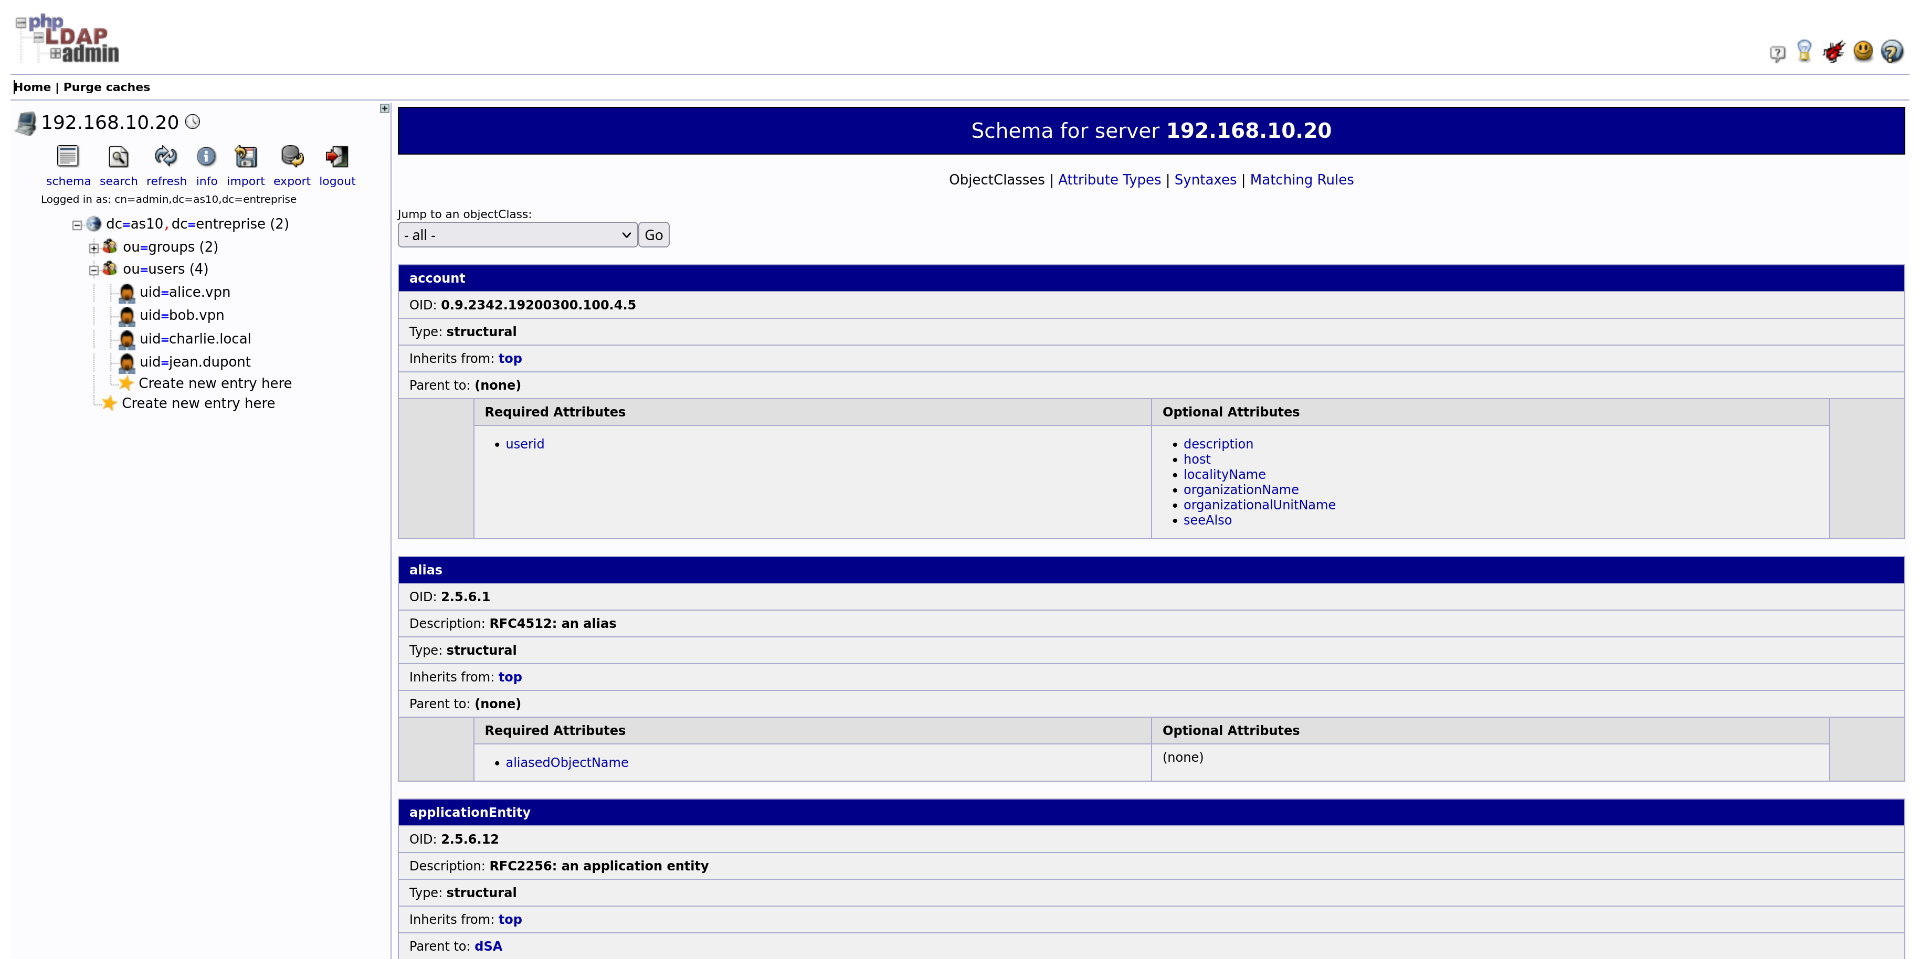
\includegraphics[width=0.7\textwidth]{image/ldap/ldap_capture_ensemble.png}
    \caption{Structure organisationnelle de l'annuaire LDAP}
    \label{fig:ldap_arbo}
\end{figure}
\begin{figure}[ht!]
    \centering
    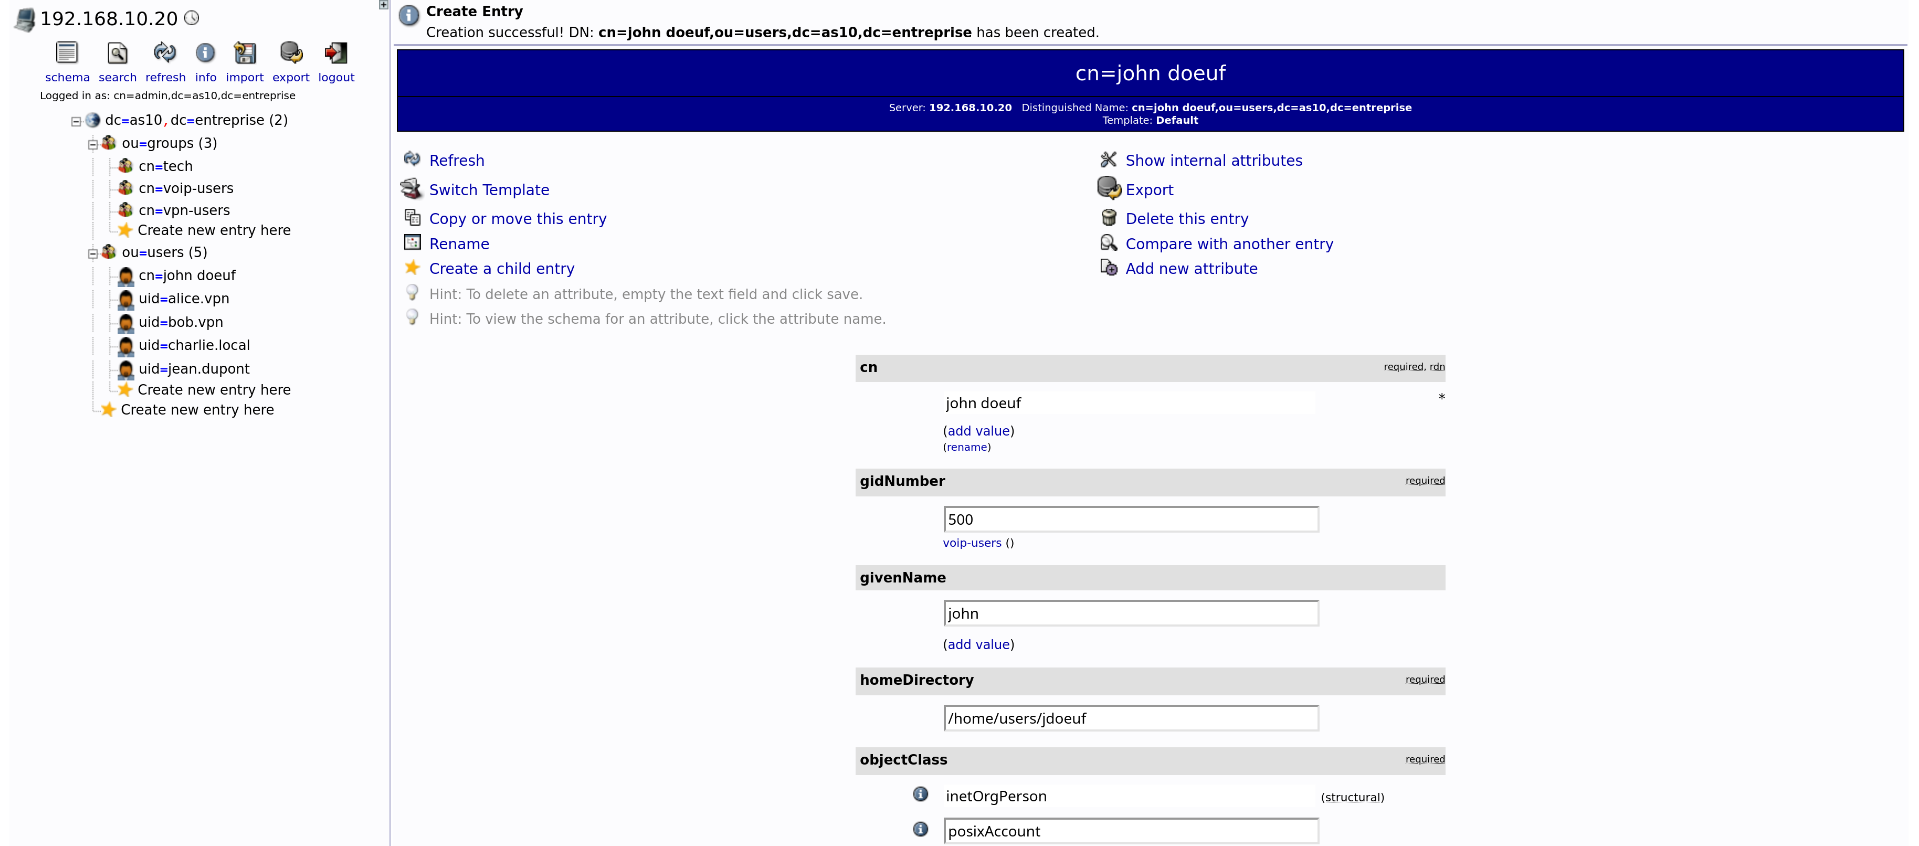
\includegraphics[width=0.7\textwidth]{image/ldap/Copie_decran_20260528_121554.png}
    \caption{Création du compte utilisateur \textit{jdoeuf}}
    \label{fig:ldap_user}
\end{figure}
\begin{figure}[ht!]
    \centering
    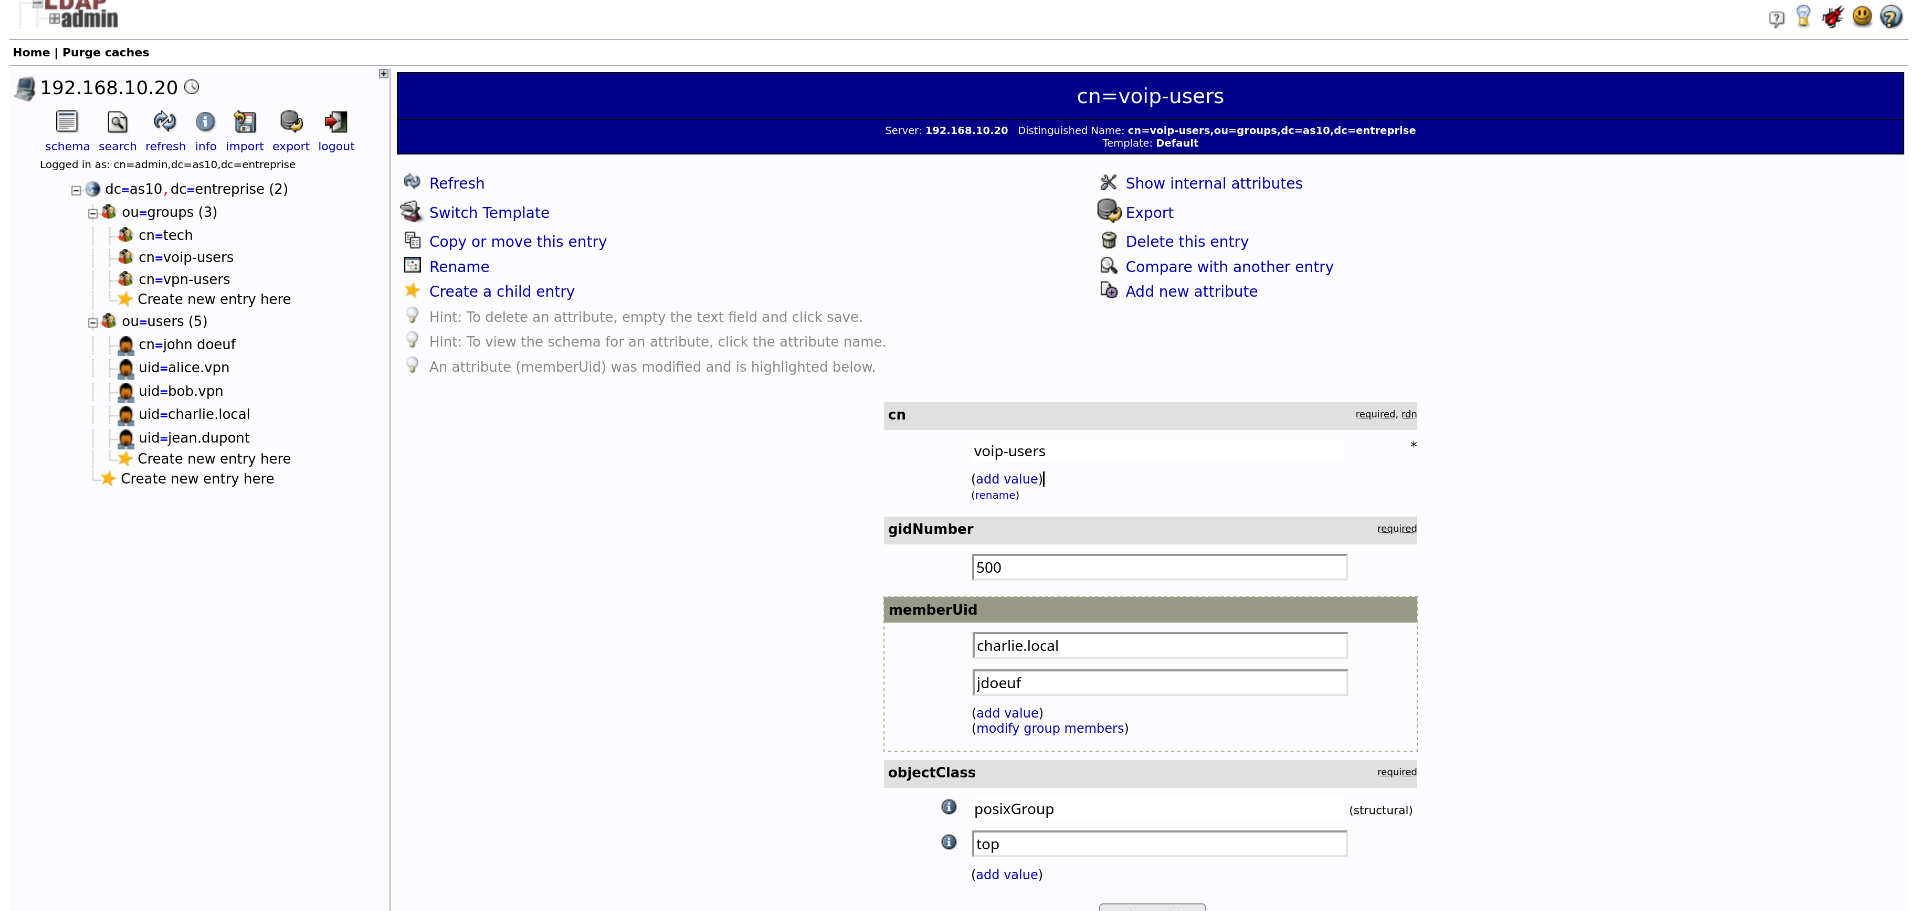
\includegraphics[width=0.7\textwidth]{image/ldap/Copie_decran_20260528_121708.png}
    \caption{Association de l'utilisateur au groupe \textit{voip-users}}
    \label{fig:ldap_group}
\end{figure}

\newpage
\subsubsection{Mise en place du DNS de l’entreprise}

La résolution de noms interne et le relais vers l’extérieur reposent sur un service DNS BIND9. Le serveur principal est hébergé dans le VLAN 10 du Datacenter à l’adresse 192.168.10.11. Il est configuré pour gérer la zone de l'entreprise \texttt{entreprise.lab}.

\paragraph{Déclaration des paramètres globaux et des zones — \texttt{/etc/bind/named.conf}}
Le fichier de configuration principal (cf Listing \ref{code:bind}) définit les règles de requêtage, active la récursivité et met en place un \textit{forwarder} pointant vers le serveur DNS de l'opérateur (AS 10) pour gérer les requêtes externes à l'entreprise.

\begin{lstlisting}[language=C, float=h, caption={/etc/bind/named.conf}, label={code:bind}]
options {
    directory "/var/cache/bind";
    listen-on { any; };
    allow-query { any; };
    recursion yes;
    dnssec-validation no;
    forwarders { 120.0.14.2; };
    forward first;
};

zone "entreprise.lab" IN {
    type master;
    file "/etc/bind/db.entreprise.lab";
};
\end{lstlisting}

\newpage
\paragraph{Fichier de zone direct — \texttt{/etc/bind/db.entreprise.lab}}
Ce fichier (cf. Listing \ref{code:bind2}) cartographie les équipements critiques de notre infrastructure en associant les noms d'hôtes aux adresses IP statiques de nos serveurs et du point d'accès externe.

\begin{lstlisting}[language=DNSZone, float=h, caption={/etc/bind/db.entreprise.lab}, label={code:bind2}]
$TTL 86400
@   IN  SOA ns1.entreprise.lab. admin.entreprise.lab. (
            2026052801 ; Serial
            3600       ; Refresh
            1800       ; Retry
            604800     ; Expire
            86400 )    ; Minimum TTL

    IN  NS  ns1.entreprise.lab.
ns1  IN  A   192.168.10.11

web      IN  A   192.168.10.10
voip     IN  A   192.168.10.12
vpn      IN  A   120.0.1.2
ldap     IN  A   192.168.10.20
ldap-ui  IN  A   192.168.10.21
\end{lstlisting}

\subsubsection{Mise en place d'un service de VoIP}

Pour répondre aux besoins de communication interne, un service de téléphonie sur IP (VoIP) a été intégré à l'architecture. La solution s'articule autour d'un autocommutateur téléphonique privé basé sur \textbf{Asterisk}, centralisé au sein du Datacenter (VLAN 10) à l'adresse 192.168.10.12. Le choix de la pile de protocoles \texttt{PJSIP} garantit une gestion moderne et sécurisée de la signalisation et des terminaux.

Côté utilisateurs, deux terminaux logiciels (softphones basés sur \texttt{baresip}) ont été déployés. Ils sont placés dans le VLAN 30, segment réseau spécifiquement dédié aux flux de téléphonie.

La mise en œuvre du service s'est déroulée en trois étapes logiques :
\begin{itemize}
    \item \textbf{Configuration des terminaux et authentification :} Chaque téléphone (PHONE-01 et PHONE-02) a été provisionné avec un compte SIP unique (extensions 100 et 200) et un mot de passe dédié pour s'authentifier auprès du serveur central.
    \item \textbf{Déclaration des points de terminaison sur le serveur :} Les téléphones ont été déclarés dans la configuration d'Asterisk en tant que \textit{endpoints} communiquant via le protocole UDP. Pour garantir la qualité et la compatibilité des flux vocaux, seuls les codecs audio standards G.711 (\texttt{alaw, ulaw}) ont été autorisés.
    \item \textbf{Mise en place du plan de numérotation (\textit{Dialplan}) :} Un contexte de routage interne a été défini sur le serveur. Il dicte la logique d'acheminement des appels : lorsqu'un utilisateur compose le numéro d'une extension, le serveur identifie le canal PJSIP correspondant et établit la mise en relation entre les deux postes téléphoniques.
\end{itemize}

\subsubsection{Mise en place d'un service applicatif supplémentaire : Serveur Web}

Un serveur Web Apache a été déployé dans le Datacenter, complétant ainsi l'infrastructure réseau avec un service applicatif supplémentaire.

Dans le cadre du projet, ce serveur héberge une page HTML simple permettant de vérifier le bon fonctionnement des différents services réseau mis en place. Même s’il s’agit principalement d’une preuve de concept, il permet de valider plusieurs aspects importants de l’infrastructure :

\begin{itemize}
    \item \textbf{Validation de la résolution DNS :} l’accès au site via le nom de domaine \texttt{web.entreprise.lab} permet de vérifier que le serveur DNS Bind9 répond correctement aux requêtes.

    \item \textbf{Validation du filtrage inter-VLAN :} ce serveur permet également de tester les règles de filtrage configurées sur le cœur de réseau avec \texttt{iptables}. Seuls les flux HTTP (TCP/80) et HTTPS (TCP/443) provenant du VLAN 20 (Clients) sont autorisés à accéder au serveur Web.
\end{itemize}

Ce service a donc servi de support de test tout au long du projet pour vérifier le bon fonctionnement du routage, du DNS ainsi que des règles de sécurité mises en place entre les VLANs.

\newpage
\subsection{Mise en œuvre du site secondaire et des accès distants}

\subsubsection{Déploiement du site secondaire et du VPN inter-sites}

Conformément aux exigences multi-sites du projet, un site d'entreprise secondaire a été intégré à l'architecture. Son infrastructure interne, bien que plus légère, reprend les mêmes principes de sécurité que le site principal, avec un réseau local protégé par un pare-feu de bordure.

Pour relier ces deux entités de manière sécurisée au travers de l'infrastructure de routage globale (via les Systèmes Autonomes), un tunnel VPN de type site-à-site a été mis en place. La technologie OpenVPN a été privilégiée pour l'établissement de ce lien. Ce tunnel chiffré relie directement le pare-feu du site principal à celui du site secondaire.

Grâce à cette implémentation et au routage configuré sur l'interface virtuelle du tunnel (\texttt{tun}), les machines du site secondaire peuvent accéder de manière transparente aux ressources centralisées du site principal (comme le serveur DNS ou la VoIP du Datacenter), comme si elles se trouvaient sur le même réseau local, tout en garantissant la confidentialité des échanges.

\subsubsection{Accès distant sécurisé pour un particulier}

En complément de l'interconnexion inter-sites, il était demandé d'offrir un accès sécurisé au réseau d'entreprise pour un utilisateur externe (particulier nomade ou télétravailleur) situé en dehors de notre infrastructure locale.

Pour ce faire, le service OpenVPN du site principal a été configuré pour accepter également des connexions de type « client-à-site ». La sécurité logique de cet accès a été renforcée en couplant le VPN avec l'annuaire LDAP de l'entreprise présenté précédemment.

Lorsqu'un particulier lance sa connexion depuis sa machine externe, son authentification est vérifiée en direct via le plugin \texttt{openvpn-auth-ldap}. Seuls les comptes possédant l'attribut \texttt{title=vpn-user} dans l'annuaire sont autorisés à monter le tunnel (correspondant aux membres du groupe \texttt{vpn-users}). Une fois authentifié, l'utilisateur nomade se voit attribuer une adresse IP virtuelle interne. Il peut ainsi interagir avec les services du Datacenter avec les mêmes restrictions de sécurité (gérées par \texttt{iptables}) que s'il était physiquement présent dans les locaux de l'entreprise.